%%%%%%
%
% $Author: Abishek,Bruna,Fedor $
% $Date: 07.10.2024 $
% $Path: ML24-02-Gait-Pattern-Recognition\report
% $Version: 1.0 $
%
%
% !TeX encoding = utf8
% !TeX root = Rename
% !TeX TXS-program:bibliography = txs:///bibtex
%
%%%%%%

\section{Arduino Nano 33 BLE Pin Configuration}

The \textbf{Arduino Nano 33 BLE} is an enhanced version of the Arduino Nano, powered by the high-performance \textbf{nRF52840 processor}. The pin configuration of this board is detailed below:\\
\vspace{1em} % Adds vertical space (adjust as needed)

\begin{figure}[h!]
	\centering
	\begin{tikzpicture}[
		pin/.style={rectangle, draw, text centered, minimum width=2.5cm, minimum height=0.8cm, font=\small},
		board/.style={draw, thick, fill=blue!20, minimum width=3cm, minimum height=15cm},
		textstyle/.style={font=\small\bfseries},
		pinpoint/.style={circle, fill=black, inner sep=0.5mm},
		every node/.style={align=center}
		]
		
		% Board
		\node[board] (board) at (0, 0) {};
		
		% USB Connector and Processor Labels
		\node[textstyle] at (0, 7) {USB};
		\node[textstyle] at (0, -7) {Processor};
		
		% Left Pins (Power, Analog, and Communication)
		\node[pin] (SCK) at (-3.5, 7) {SCK};
		\node[pin] (3V3) at (-3.5, 6) {+3.3V OUT};
		\node[pin] (AREF) at (-3.5, 5) {AREF};
		\node[pin] (A0) at (-3.5, 4) {A0};
		\node[pin] (A1) at (-3.5, 3) {A1};
		\node[pin] (A2) at (-3.5, 2) {A2};
		\node[pin] (A3) at (-3.5, 1) {A3};
		\node[pin] (A4) at (-3.5, 0) {A4};
		\node[pin] (A5) at (-3.5, -1) {A5};
		\node[pin] (A6) at (-3.5, -2) {A6};
		\node[pin] (A7) at (-3.5, -3) {A7};
		\node[pin] (5V) at (-3.5, -4) {+5V OUT};
		\node[pin] (RESETL) at (-3.5, -5) {RESET};
		\node[pin] (GNDL) at (-3.5, -6) {GND};
		\node[pin] (VIN) at (-3.5, -7) {VIN IN};
		
		% Right Pins (Digital, SPI, and UART)
		\node[pin] (D12) at (3.5, 7) {D12};
		\node[pin] (D11) at (3.5, 6) {D11};
		\node[pin] (D10) at (3.5, 5) {D10};
		\node[pin] (D9) at (3.5, 4) {D9};
		\node[pin] (D8) at (3.5, 3) {D8};
		\node[pin] (D7) at (3.5, 2) {D7};
		\node[pin] (D6) at (3.5, 1) {D6};
		\node[pin] (D5) at (3.5, 0) {D5};
		\node[pin] (D4) at (3.5, -1) {D4};
		\node[pin] (D3) at (3.5, -2) {D3};
		\node[pin] (D2) at (3.5, -3) {D2};
		\node[pin] (GNDR) at (3.5, -4) {GND};
		\node[pin] (RESETR) at (3.5, -5) {RESET};
		\node[pin] (RX) at (3.5, -6) {RX};
		\node[pin] (TX) at (3.5, -7) {TX};
		
		% Add pin values (left for left pins, right for right pins)
		\node[left=0.5cm of SCK] {\small P0.13};
		\node[left=0.5cm of A0] {\small P0.04};
		\node[left=0.5cm of A1] {\small P0.05};
		\node[left=0.5cm of A2] {\small P0.30};
		\node[left=0.5cm of A3] {\small P0.29};
		\node[left=0.5cm of A4] {\small P0.31};
		\node[left=0.5cm of A5] {\small P0.02};
		\node[left=0.5cm of A6] {\small P0.28};
		\node[left=0.5cm of A7] {\small P0.03};
		
		\node[right=0.5cm of D12] {\small P1.08};
		\node[right=0.5cm of D11] {\small P1.01};
		\node[right=0.5cm of D10] {\small P1.02};
		\node[right=0.5cm of D9] {\small P0.27};
		\node[right=0.5cm of D8] {\small P0.21};
		\node[right=0.5cm of D7] {\small P0.23};
		\node[right=0.5cm of D6] {\small P1.14};
		\node[right=0.5cm of D5] {\small P1.13};
		\node[right=0.5cm of D4] {\small P1.15};
		\node[right=0.5cm of D3] {\small P1.12};
		\node[right=0.5cm of D2] {\small P1.11};
		\node[right=0.5cm of RX] {\small P1.10};
		\node[right=0.5cm of TX] {\small P1.03};
		
		% Connections (Fixed vertical alignment for corresponding pins)
		% Left Pins to Board
		\foreach \i/\y in {SCK/7, 3V3/6, AREF/5, A0/4, A1/3, A2/2, A3/1, A4/0, A5/-1, A6/-2, A7/-3, 5V/-4, RESETL/-5, GNDL/-6, VIN/-7} {
			\draw (\i.east) -- (-1.5, \y) node[pinpoint] {};
		}
		
		% Right Pins to Board
		\foreach \i/\y in {D12/7, D11/6, D10/5, D9/4, D8/3, D7/2, D6/1, D5/0, D4/-1, D3/-2, D2/-3, GNDR/-4, RESETR/-5, RX/-6, TX/-7} {
			\draw (\i.west) -- (1.5, \y) node[pinpoint] {};
		}
		
		% Add "Top View" Label
		\node[textstyle] at (0, -8.5) {\textbf{Top View}};
		
	\end{tikzpicture}
	\caption{Arduino Nano 33 BLE Pin Configuration}
	\label{fig:arduino_pin_config}
\end{figure}

\subsubsection{Digital Pins}
The board includes \textbf{14 digital I/O pins}, which can either function as inputs or outputs, depending on the application. These pins operate in two states:
\\ \\
\vspace{1em} % Adds vertical space (adjust as needed)
\begin{figure}[h!]
	\centering
	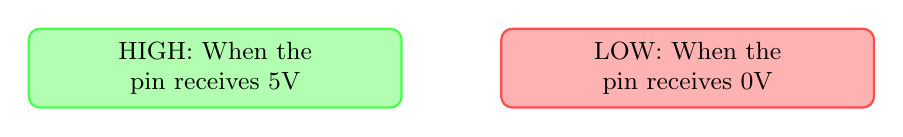
\begin{tikzpicture}[
		node distance=2cm, 
		every node/.style={align=center, font=\bfseries},
		state/.style={rectangle, draw, thick, text width=4.5cm, rounded corners, minimum height=1cm, font=\small},
		high/.style={state, fill=green!30, draw=green!70},
		low/.style={state, fill=red!30, draw=red!70}
		]
		
		% Left Figure: HIGH State
		\node[high] (high) at (2,0) {HIGH: When the pin receives 5V};
		
		% Right Figure: LOW State
		\node[low] (low) at (8,0) {LOW: When the pin receives 0V};
		
	\end{tikzpicture}
	\caption{Digital Pin States: HIGH and LOW Logic Levels}
	\label{fig:digital_pin_states}
\end{figure}

\subsubsection{Analog Pins}
There are \textbf{8 analog pins (A0–A7)} on the board. Unlike digital pins, analog pins can accept a range of values, measuring voltages between \textbf{0V and 3.3V}. The measured voltage is then converted into a corresponding digital value using the \textbf{12-bit ADC (Analog-to-Digital Converter)}, resulting in a range of values from \textbf{0 to 4095}. These pins are commonly used for capturing variable signals, such as sensor outputs. Exceeding 3.3V on these pins can damage the microcontroller, so higher input voltages require a voltage divider or level shifter to ensure safe operation.
\\ \\
\vspace{1em} % Adds vertical space (adjust as needed)
\begin{figure}[h!]
	\centering
	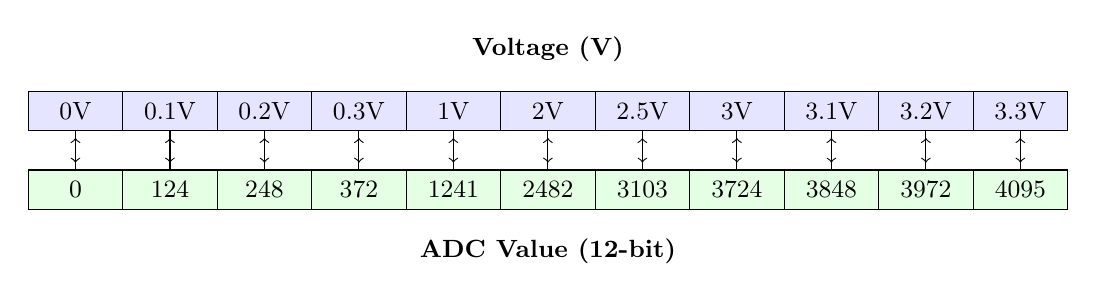
\begin{tikzpicture}[
		every node/.style={font=\small},
		voltage/.style={draw, fill=blue!10, minimum height=0.5cm, minimum width=1.2cm, align=center},
		adc/.style={draw, fill=green!10, minimum height=0.5cm, minimum width=1.2cm, align=center}
		]
		
		% Draw Voltage Levels
		\node[voltage] (v0) at (0, 0) {0V};
		\node[voltage] (v1) at (1.2, 0) {0.1V};
		\node[voltage] (v2) at (2.4, 0) {0.2V};
		\node[voltage] (v3) at (3.6, 0) {0.3V};
		\node[voltage] (v4) at (4.8, 0) {1V};
		\node[voltage] (v5) at (6.0, 0) {2V};
		\node[voltage] (v6) at (7.2, 0) {2.5V};
		\node[voltage] (v7) at (8.4, 0) {3V};
		\node[voltage] (v8) at (9.6, 0) {3.1V};
		\node[voltage] (v9) at (10.8, 0) {3.2V};
		\node[voltage] (v10) at (12.0, 0) {3.3V};
		
		% Draw ADC Values Below Voltage Levels
		\node[adc] (a0) at (0, -1) {0};
		\node[adc] (a1) at (1.2, -1) {124};
		\node[adc] (a2) at (2.4, -1) {248};
		\node[adc] (a3) at (3.6, -1) {372};
		\node[adc] (a4) at (4.8, -1) {1241};
		\node[adc] (a5) at (6.0, -1) {2482};
		\node[adc] (a6) at (7.2, -1) {3103};
		\node[adc] (a7) at (8.4, -1) {3724};
		\node[adc] (a8) at (9.6, -1) {3848};
		\node[adc] (a9) at (10.8, -1) {3972};
		\node[adc] (a10) at (12.0, -1) {4095};
		
		% Add Arrows for Clarity
		\foreach \x in {v0, v1, v2, v3, v4, v5, v6, v7, v8, v9, v10} {
			\draw[->] (\x.south) -- +(0, -0.4);
		}
		\foreach \x in {a0, a1, a2, a3, a4, a5, a6, a7, a8, a9, a10} {
			\draw[->] (\x.north) -- +(0, 0.4);
		}
		
		% Add Axis Label
		\node[above=0.5cm] at (6, 0) {\textbf{Voltage (V)}};
		\node[below=1cm] at (6, -0.5) {\textbf{ADC Value (12-bit)}};
		
	\end{tikzpicture}
	\caption{Mapping of Voltage Levels to ADC Values in the Arduino Nano 33 BLE Sense Rev 2}
	\label{fig:adc_mapping}
\end{figure}

\subsubsection{Pulse Width Modulation (PWM)}

The Arduino Nano 33 BLE Sense Rev 2 supports \textbf{Pulse Width Modulation (PWM)} on specific digital pins, enabling the generation of analog-like signals through digital techniques. By rapidly toggling between \textbf{HIGH} and \textbf{LOW} states, PWM produces a signal with a variable \textbf{duty cycle}, determining the effective voltage output. Common applications include motor control, LED dimming, and audio tone generation. The \texttt{analogWrite()} function facilitates straightforward PWM implementation. 
\\ \\
\vspace{1em} % Adds vertical space (adjust as needed)
\begin{figure}[h!]
	\centering
	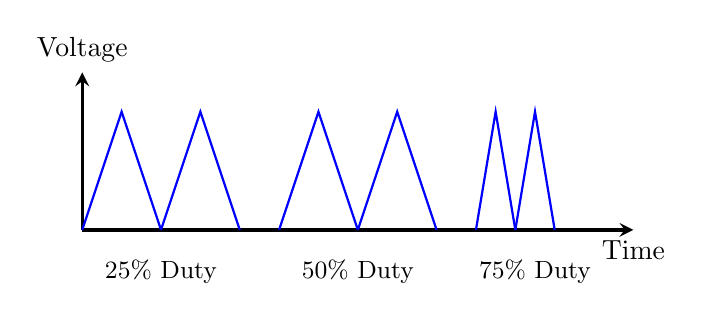
\begin{tikzpicture}[
		axis/.style={very thick, ->, >=stealth},
		wave/.style={thick, draw=blue},
		label/.style={font=\small, anchor=north}
		]
		
		% Draw axes
		\draw[axis] (0, 0) -- (7, 0) node[anchor=north] {Time};
		\draw[axis] (0, 0) -- (0, 2) node[anchor=south] {Voltage};
		
		% Draw PWM waveforms
		% 25% Duty Cycle
		\draw[wave] (0, 0) -- (0.5, 1.5) -- (1, 0);
		\draw[wave] (1, 0) -- (1.5, 1.5) -- (2, 0);
		
		% 50% Duty Cycle
		\draw[wave] (2.5, 0) -- (3, 1.5) -- (3.5, 0);
		\draw[wave] (3.5, 0) -- (4, 1.5) -- (4.5, 0);
		
		% 75% Duty Cycle
		\draw[wave] (5, 0) -- (5.25, 1.5) -- (5.5, 0);
		\draw[wave] (5.5, 0) -- (5.75, 1.5) -- (6, 0);
		
		% Add labels for duty cycles
		\node[label] at (1, -0.25) {25\% Duty};
		\node[label] at (3.5, -0.25) {50\% Duty};
		\node[label] at (5.75, -0.25) {75\% Duty};
		
	\end{tikzpicture}
	\caption{PWM Waveforms with Different Duty Cycles}
	\label{fig:pwm_waveforms}
\end{figure}

\subsubsection{SPI Pins}
The Arduino Nano 33 BLE supports \textbf{SPI (Serial Peripheral Interface) communication}, which facilitates data exchange between the microcontroller and peripheral devices such as sensors or shift registers.
\\ \\
\vspace{1em} % Adds vertical space (adjust as needed)
\begin{figure}[h!]
	\centering
	\begin{tikzpicture}[
		device/.style={rectangle, draw, fill=green!20, text centered, minimum width=3cm, minimum height=2.5cm, font=\small\bfseries},
		pin/.style={rectangle, draw, fill=blue!10, minimum width=2cm, minimum height=1cm, align=center, font=\small},
		arrow/.style={->, thick},
		label/.style={font=\small},
		every node/.style={align=center}
		]
		
		% Master Device (Microcontroller)
		\node[device] (master) at (-3, 0) {Microcontroller\\(Master)};
		
		% Slave Device (Peripheral)
		\node[device, fill=red!20] (slave) at (10, 0) {Peripheral Device\\(Slave)};
		
		% Master Pins
		\node[pin, right=2cm of master.north] (sck) {SCK (D13)};
		\node[pin, below=0.5cm of sck] (mosi) {MOSI (D11)};
		\node[pin, below=0.5cm of mosi] (miso) {MISO (D12)};
		\node[pin, below=0.5cm of miso] (ss) {SS (D10)};
		
		% Slave Pins
		\node[pin, left=2cm of slave.north] (sclk_slave) {SCK};
		\node[pin, below=0.5cm of sclk_slave] (sdi) {SDI};
		\node[pin, below=0.5cm of sdi] (sdo) {SDO};
		\node[pin, below=0.5cm of sdo] (cs) {CS};
		
		% Connections
		\draw[arrow] (sck.east) -- (sclk_slave.west) node[midway, above] {Clock (SCLK)};
		\draw[arrow] (mosi.east) -- (sdi.west) node[midway, above] {Data to Slave (SDI)};
		\draw[arrow] (sdo.west) -- (miso.east) node[midway, above] {Data to Master (SDO)};
		\draw[arrow] (ss.east) -- (cs.west) node[midway, above] {Chip Select (CS)};
		
	\end{tikzpicture}
	\caption{SPI Communication between Master and Slave Devices}
	\label{fig:spi_communication}
\end{figure}
\begin{itemize}
	\item \textbf{MISO (Master Input Slave Output):} Receives data from peripherals.
	\item \textbf{MOSI (Master Output Slave Input):} Sends data to peripherals.
\end{itemize}

\subsubsection{I2C Pins}
The board features the \textbf{I2C protocol}, a two-wire communication standard widely used for connecting multiple devices.
\begin{figure}[h!]
	\centering
	% Arduino as Slave
	\begin{subfigure}[b]{0.45\textwidth}
		\centering
		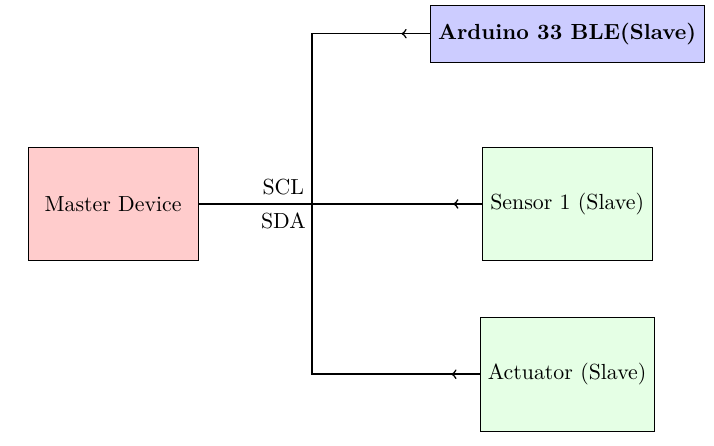
\includegraphics[width=\textwidth]{Images/arduinoSlavei2c.png}
		\caption{Arduino as Slave in I2C Communication}
		\label{fig:arduino_slave}
	\end{subfigure}
	\hfill
	% Arduino as Master
	\begin{subfigure}[b]{0.45\textwidth}
		\centering
		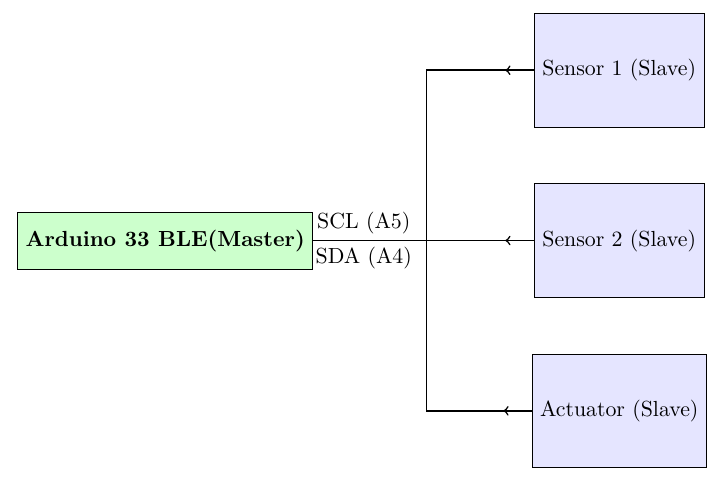
\includegraphics[width=\textwidth]{Images/arduinoMasteri2c.png}
		\caption{Arduino as Master in I2C Communication}
		\label{fig:arduino_master}
	\end{subfigure}
	\caption{I2C Communication with Arduino in Master and Slave Configurations.}
	\label{fig:i2c_communication}
\end{figure}
\begin{itemize}
	\item \textbf{MISO (Master Input Slave Output):} Receives data from peripherals.
	\item \textbf{MOSI (Master Output Slave Input):} Sends data to peripherals.
\end{itemize}
\begin{itemize}
	\item \textbf{SCL (Serial Clock Line):} Synchronizes data transfer.
	\item \textbf{SDA (Serial Data Line):} Transmits and receives data.
\end{itemize} 




\subsubsection{UART Pins}
The board also includes support for the \textbf{UART (Universal Asynchronous Receiver-Transmitter) protocol}, which enables serial communication.
\begin{itemize}
	\item \textbf{Rx (Receive):} Used to receive serial data.
	\item \textbf{Tx (Transmit):} Used to send serial data.
\end{itemize}

\subsubsection{External Interrupt Pins}
All \textbf{digital pins} can be configured as \textbf{external interrupt pins}. These are used to pause the main program when an urgent task or event occurs, ensuring immediate response to critical inputs.

\subsubsection{Special Pins}
\begin{itemize}
	\item \textbf{LED (Pin 13):} The board features a built-in LED connected to \textbf{pin 13}, often used for debugging or indicating system states.
	\item \textbf{AREF Pin:} The \textbf{Analog Reference (AREF)} pin is used to provide a reference voltage for analog inputs, ensuring precise readings.
\end{itemize}

This pin configuration makes the Arduino Nano 33 BLE a versatile and powerful tool for a wide range of embedded applications.